% Options for packages loaded elsewhere
\PassOptionsToPackage{unicode}{hyperref}
\PassOptionsToPackage{hyphens}{url}
%
\documentclass[
]{article}
\usepackage{amsmath,amssymb}
\usepackage{lmodern}
\usepackage{ifxetex,ifluatex}
\ifnum 0\ifxetex 1\fi\ifluatex 1\fi=0 % if pdftex
  \usepackage[T1]{fontenc}
  \usepackage[utf8]{inputenc}
  \usepackage{textcomp} % provide euro and other symbols
\else % if luatex or xetex
  \usepackage{unicode-math}
  \defaultfontfeatures{Scale=MatchLowercase}
  \defaultfontfeatures[\rmfamily]{Ligatures=TeX,Scale=1}
\fi
% Use upquote if available, for straight quotes in verbatim environments
\IfFileExists{upquote.sty}{\usepackage{upquote}}{}
\IfFileExists{microtype.sty}{% use microtype if available
  \usepackage[]{microtype}
  \UseMicrotypeSet[protrusion]{basicmath} % disable protrusion for tt fonts
}{}
\makeatletter
\@ifundefined{KOMAClassName}{% if non-KOMA class
  \IfFileExists{parskip.sty}{%
    \usepackage{parskip}
  }{% else
    \setlength{\parindent}{0pt}
    \setlength{\parskip}{6pt plus 2pt minus 1pt}}
}{% if KOMA class
  \KOMAoptions{parskip=half}}
\makeatother
\usepackage{xcolor}
\IfFileExists{xurl.sty}{\usepackage{xurl}}{} % add URL line breaks if available
\IfFileExists{bookmark.sty}{\usepackage{bookmark}}{\usepackage{hyperref}}
\hypersetup{
  pdftitle={Soybean Analysis},
  pdfauthor={Efoli Matthew},
  hidelinks,
  pdfcreator={LaTeX via pandoc}}
\urlstyle{same} % disable monospaced font for URLs
\usepackage[margin=1in]{geometry}
\usepackage{color}
\usepackage{fancyvrb}
\newcommand{\VerbBar}{|}
\newcommand{\VERB}{\Verb[commandchars=\\\{\}]}
\DefineVerbatimEnvironment{Highlighting}{Verbatim}{commandchars=\\\{\}}
% Add ',fontsize=\small' for more characters per line
\usepackage{framed}
\definecolor{shadecolor}{RGB}{248,248,248}
\newenvironment{Shaded}{\begin{snugshade}}{\end{snugshade}}
\newcommand{\AlertTok}[1]{\textcolor[rgb]{0.94,0.16,0.16}{#1}}
\newcommand{\AnnotationTok}[1]{\textcolor[rgb]{0.56,0.35,0.01}{\textbf{\textit{#1}}}}
\newcommand{\AttributeTok}[1]{\textcolor[rgb]{0.77,0.63,0.00}{#1}}
\newcommand{\BaseNTok}[1]{\textcolor[rgb]{0.00,0.00,0.81}{#1}}
\newcommand{\BuiltInTok}[1]{#1}
\newcommand{\CharTok}[1]{\textcolor[rgb]{0.31,0.60,0.02}{#1}}
\newcommand{\CommentTok}[1]{\textcolor[rgb]{0.56,0.35,0.01}{\textit{#1}}}
\newcommand{\CommentVarTok}[1]{\textcolor[rgb]{0.56,0.35,0.01}{\textbf{\textit{#1}}}}
\newcommand{\ConstantTok}[1]{\textcolor[rgb]{0.00,0.00,0.00}{#1}}
\newcommand{\ControlFlowTok}[1]{\textcolor[rgb]{0.13,0.29,0.53}{\textbf{#1}}}
\newcommand{\DataTypeTok}[1]{\textcolor[rgb]{0.13,0.29,0.53}{#1}}
\newcommand{\DecValTok}[1]{\textcolor[rgb]{0.00,0.00,0.81}{#1}}
\newcommand{\DocumentationTok}[1]{\textcolor[rgb]{0.56,0.35,0.01}{\textbf{\textit{#1}}}}
\newcommand{\ErrorTok}[1]{\textcolor[rgb]{0.64,0.00,0.00}{\textbf{#1}}}
\newcommand{\ExtensionTok}[1]{#1}
\newcommand{\FloatTok}[1]{\textcolor[rgb]{0.00,0.00,0.81}{#1}}
\newcommand{\FunctionTok}[1]{\textcolor[rgb]{0.00,0.00,0.00}{#1}}
\newcommand{\ImportTok}[1]{#1}
\newcommand{\InformationTok}[1]{\textcolor[rgb]{0.56,0.35,0.01}{\textbf{\textit{#1}}}}
\newcommand{\KeywordTok}[1]{\textcolor[rgb]{0.13,0.29,0.53}{\textbf{#1}}}
\newcommand{\NormalTok}[1]{#1}
\newcommand{\OperatorTok}[1]{\textcolor[rgb]{0.81,0.36,0.00}{\textbf{#1}}}
\newcommand{\OtherTok}[1]{\textcolor[rgb]{0.56,0.35,0.01}{#1}}
\newcommand{\PreprocessorTok}[1]{\textcolor[rgb]{0.56,0.35,0.01}{\textit{#1}}}
\newcommand{\RegionMarkerTok}[1]{#1}
\newcommand{\SpecialCharTok}[1]{\textcolor[rgb]{0.00,0.00,0.00}{#1}}
\newcommand{\SpecialStringTok}[1]{\textcolor[rgb]{0.31,0.60,0.02}{#1}}
\newcommand{\StringTok}[1]{\textcolor[rgb]{0.31,0.60,0.02}{#1}}
\newcommand{\VariableTok}[1]{\textcolor[rgb]{0.00,0.00,0.00}{#1}}
\newcommand{\VerbatimStringTok}[1]{\textcolor[rgb]{0.31,0.60,0.02}{#1}}
\newcommand{\WarningTok}[1]{\textcolor[rgb]{0.56,0.35,0.01}{\textbf{\textit{#1}}}}
\usepackage{graphicx}
\makeatletter
\def\maxwidth{\ifdim\Gin@nat@width>\linewidth\linewidth\else\Gin@nat@width\fi}
\def\maxheight{\ifdim\Gin@nat@height>\textheight\textheight\else\Gin@nat@height\fi}
\makeatother
% Scale images if necessary, so that they will not overflow the page
% margins by default, and it is still possible to overwrite the defaults
% using explicit options in \includegraphics[width, height, ...]{}
\setkeys{Gin}{width=\maxwidth,height=\maxheight,keepaspectratio}
% Set default figure placement to htbp
\makeatletter
\def\fps@figure{htbp}
\makeatother
\setlength{\emergencystretch}{3em} % prevent overfull lines
\providecommand{\tightlist}{%
  \setlength{\itemsep}{0pt}\setlength{\parskip}{0pt}}
\setcounter{secnumdepth}{-\maxdimen} % remove section numbering
\ifluatex
  \usepackage{selnolig}  % disable illegal ligatures
\fi

\title{Soybean Analysis}
\author{Efoli Matthew}
\date{11/08/2021}

\begin{document}
\maketitle

\hypertarget{activities}{%
\subsubsection{Activities}\label{activities}}

\begin{enumerate}
\def\labelenumi{\arabic{enumi}.}
\tightlist
\item
  Create a new Rstudio Project
\item
  Create and save a new analysis.Rmd file
\item
  Open the analysis.Rmd file and start working on it
\end{enumerate}

\hypertarget{import-the-data-from-a-google-sheet-library-gsheet.-give-a-name-to-the-dataframe-object-httpsdocs.google.comspreadsheetsd16bdpdimy6gysrkahfiem_y5hy13d3pskfgjaybjvdnwedituspsharing}{%
\paragraph{\texorpdfstring{4. Import the data from a google sheet
(library gsheet). Give a name to the dataframe object
(\url{https://docs.google.com/spreadsheets/d/16BdPdimy6GYsrkahFiEM_y5Hy13D3psKfGJayBjVdNw/edit?usp=sharing}
)}{4. Import the data from a google sheet (library gsheet). Give a name to the dataframe object (https://docs.google.com/spreadsheets/d/16BdPdimy6GYsrkahFiEM\_y5Hy13D3psKfGJayBjVdNw/edit?usp=sharing )}}\label{import-the-data-from-a-google-sheet-library-gsheet.-give-a-name-to-the-dataframe-object-httpsdocs.google.comspreadsheetsd16bdpdimy6gysrkahfiem_y5hy13d3pskfgjaybjvdnwedituspsharing}}

\hypertarget{check-the-structure-of-the-data-set-glimpse}{%
\subsection{5. Check the structure of the data set
(glimpse())}\label{check-the-structure-of-the-data-set-glimpse}}

\begin{verbatim}
## function (..., list = character(), package = NULL, lib.loc = NULL, verbose = getOption("verbose"), 
##     envir = .GlobalEnv, overwrite = TRUE)
\end{verbatim}

\hypertarget{save-the-data.frame-as-data.csv-in-the-project-directory}{%
\subsection{6. Save the data.frame as data.csv in the project
directory}\label{save-the-data.frame-as-data.csv-in-the-project-directory}}

\begin{Shaded}
\begin{Highlighting}[]
\CommentTok{\#write.csv(data,\textquotesingle{}data.csv\textquotesingle{})}
\end{Highlighting}
\end{Shaded}

\hypertarget{open-the-data-in-the-data.csv-file-and-assign-to-a-new-dataframe}{%
\subsection{7. Open the data in the data.csv file and assign to a new
dataframe}\label{open-the-data-in-the-data.csv-file-and-assign-to-a-new-dataframe}}

\begin{Shaded}
\begin{Highlighting}[]
\NormalTok{soybean }\OtherTok{\textless{}{-}} \FunctionTok{data.frame}\NormalTok{(}\FunctionTok{read.csv}\NormalTok{(}\StringTok{"data.csv"}\NormalTok{, }\AttributeTok{header =}\NormalTok{ T))}
\FunctionTok{head}\NormalTok{(soybean)}
\end{Highlighting}
\end{Shaded}

\begin{verbatim}
##   X study year    location state block         treat
## 1 1   424 2020 CAMPO VERDE    MT     1 Aproach Prima
## 2 2   424 2020 CAMPO VERDE    MT     2 Aproach Prima
## 3 3   424 2020 CAMPO VERDE    MT     3 Aproach Prima
## 4 4   424 2020 CAMPO VERDE    MT     4 Aproach Prima
## 5 5   424 2020 CAMPO VERDE    MT     1        Ativum
## 6 6   424 2020 CAMPO VERDE    MT     2        Ativum
##                                             ai sev  yld
## 1                picoxystrobin + cyproconazole  28 3060
## 2                picoxystrobin + cyproconazole  28 3145
## 3                picoxystrobin + cyproconazole  47 3104
## 4                picoxystrobin + cyproconazole  50 3072
## 5 epoxiconazole + fluxapiroxade+pyraclostrobin  38 3699
## 6 epoxiconazole + fluxapiroxade+pyraclostrobin  35 3498
\end{verbatim}

\hypertarget{start-exploring-the-data.-first-subset-the-trials-and-create-four-different-dataframes-one-for-each-trial-there-are-four-trials}{%
\subsection{8. Start exploring the data. First, subset the trials and
create four different dataframes, one for each trial (there are four
trials)}\label{start-exploring-the-data.-first-subset-the-trials-and-create-four-different-dataframes-one-for-each-trial-there-are-four-trials}}

The Soybean data set is subset into 4 different data frames by trials.

\begin{verbatim}
## [1] "424" "425" "426" "427"
\end{verbatim}

\begin{verbatim}
## 'data.frame':    112 obs. of  10 variables:
##  $ X       : int  1 2 3 4 5 6 7 8 9 10 ...
##  $ study   : int  424 424 424 424 424 424 424 424 424 424 ...
##  $ year    : int  2020 2020 2020 2020 2020 2020 2020 2020 2020 2020 ...
##  $ location: chr  "CAMPO VERDE" "CAMPO VERDE" "CAMPO VERDE" "CAMPO VERDE" ...
##  $ state   : chr  "MT" "MT" "MT" "MT" ...
##  $ block   : Factor w/ 4 levels "1","2","3","4": 1 2 3 4 1 2 3 4 1 2 ...
##  $ treat   : Factor w/ 7 levels "Aproach Prima",..: 1 1 1 1 2 2 2 2 3 3 ...
##  $ ai      : chr  "picoxystrobin + cyproconazole" "picoxystrobin + cyproconazole" "picoxystrobin + cyproconazole" "picoxystrobin + cyproconazole" ...
##  $ sev     : int  28 28 47 50 38 35 45 40 55 70 ...
##  $ yld     : int  3060 3145 3104 3072 3699 3498 3420 3387 2658 2994 ...
\end{verbatim}

\hypertarget{produce-plots-to-visualize-the-response-variables}{%
\subsection{9. Produce plots to visualize the response
variables}\label{produce-plots-to-visualize-the-response-variables}}

We have two response variables namely; yield and severity. We would
present the yield and severity response variables using bar charts.

\hypertarget{data-visualization-for-trial-1}{%
\subsubsection{Data Visualization for Trial
1}\label{data-visualization-for-trial-1}}

The table shows the soybean mean yield, standard deviation by treatment
for trial 1. The mean of the blocks is estimated as the yield for each
treatment.

\begin{verbatim}
## Loading required package: plyr
\end{verbatim}

\begin{verbatim}
## ------------------------------------------------------------------------------
\end{verbatim}

\begin{verbatim}
## You have loaded plyr after dplyr - this is likely to cause problems.
## If you need functions from both plyr and dplyr, please load plyr first, then dplyr:
## library(plyr); library(dplyr)
\end{verbatim}

\begin{verbatim}
## ------------------------------------------------------------------------------
\end{verbatim}

\begin{verbatim}
## 
## Attaching package: 'plyr'
\end{verbatim}

\begin{verbatim}
## The following object is masked from 'package:ggpubr':
## 
##     mutate
\end{verbatim}

\begin{verbatim}
## The following objects are masked from 'package:dplyr':
## 
##     arrange, count, desc, failwith, id, mutate, rename, summarise,
##     summarize
\end{verbatim}

\begin{verbatim}
##           treat     yld        sd
## 1 Aproach Prima 3095.25  38.01206
## 2        Ativum 3501.00 139.96428
## 3       Control 2925.25 180.15063
## 4        Elatus 3283.25 195.30382
## 5           FOX 3405.75 110.29166
## 6         Fusao 3445.50 155.22135
## 7      Vessarya 3247.25 226.84264
\end{verbatim}

From the above table, Soybean treated with treatments, Ativum, Fusao,
FOX have the highest average yield; 3501, 3445.50 and 3405.75
respectively.

The table shows the soybean mean severity, standard deviation by
treatment for the trial 1. The mean of the blocks is estimated as the
yield for each treatment.

\begin{verbatim}
##           treat   sev        sd
## 1 Aproach Prima 38.25 11.898879
## 2        Ativum 39.50  4.203173
## 3       Control 65.50  7.593857
## 4        Elatus 29.50  5.259911
## 5           FOX 33.50  3.415650
## 6         Fusao 29.50  8.346656
## 7      Vessarya 28.25  2.362908
\end{verbatim}

From the above table, the control, and Soybean treated with treatments,
Ativum, Aproach Prima have the highest average severity; 65.50, 39.50,
38.25 respectively.

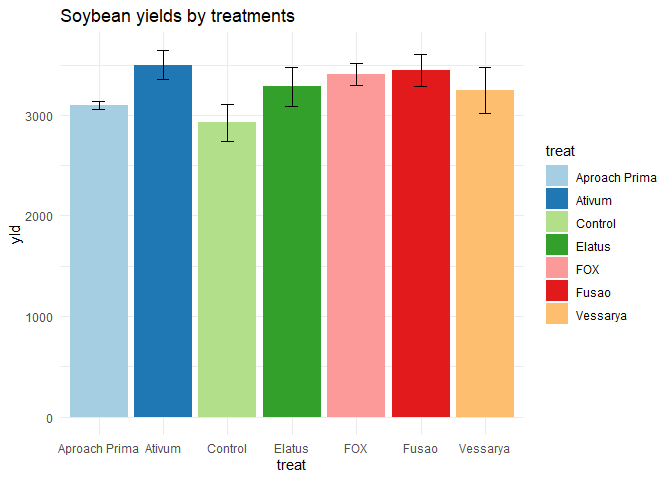
\includegraphics{Trails-of-4-trials_files/figure-latex/dviz1-1.pdf}

From the above chart, Soybean treated with treatments, Ativum, Fusao,
FOX have the highest average yield; 3501, 3445.50 and 3405.75
respectively.

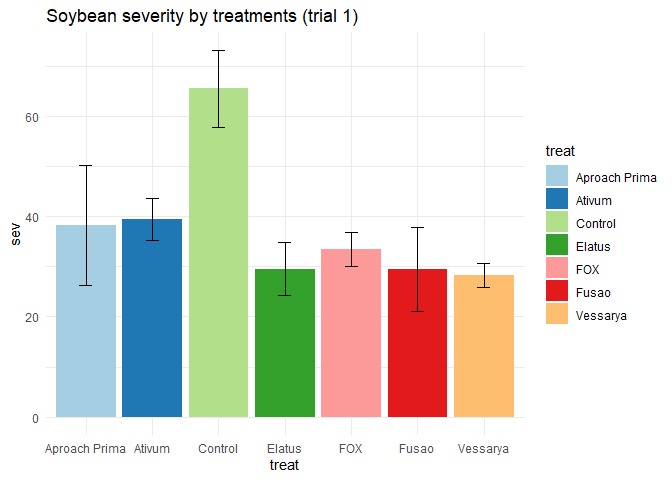
\includegraphics{Trails-of-4-trials_files/figure-latex/dviz1b-1.pdf} The
chart above shows that the control, and Soybean treated with treatments,
Ativum, Aproach Prima have the highest average severity; 65.50, 39.50,
38.25 respectively.

\hypertarget{data-visualization-for-trial-2}{%
\subsubsection{Data visualization for trial
2}\label{data-visualization-for-trial-2}}

\begin{verbatim}
##           treat     yld       sd
## 1 Aproach Prima 4114.25 238.6872
## 2        Ativum 3995.75 121.5000
## 3       Control 4023.25 101.1645
## 4        Elatus 3912.25 223.6878
## 5           FOX 4157.25 291.1877
## 6         Fusao 4063.75 172.9824
## 7      Vessarya 4232.00 255.5113
\end{verbatim}

From the above table, Soybean treated with treatments, Vessarya, FOX,
Aproach Prima have the highest average yield; 4232, 4147.25, and 4114.25
respectively.

\begin{verbatim}
##           treat   sev       sd
## 1 Aproach Prima  5.00 0.000000
## 2        Ativum  6.00 1.154701
## 3       Control 38.25 2.362908
## 4        Elatus  7.25 2.061553
## 5           FOX  5.00 1.632993
## 6         Fusao  6.75 2.362908
## 7      Vessarya  6.00 1.154701
\end{verbatim}

The above table shows that Control(38.25) and treatments; Elatus(7.25)
and Fusao(6.75) had the highest severity.

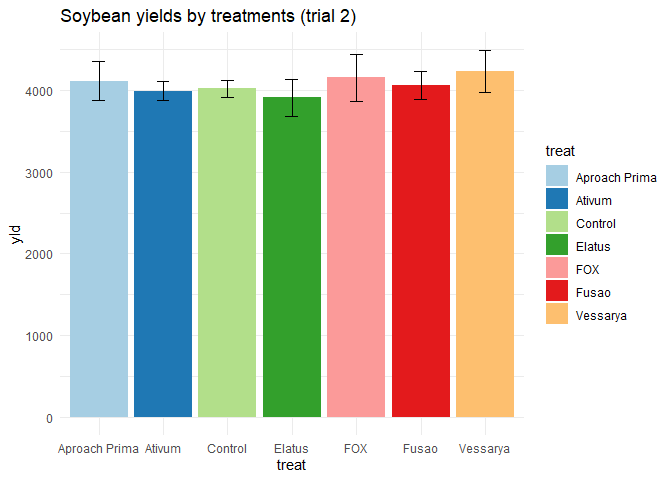
\includegraphics{Trails-of-4-trials_files/figure-latex/dviz2-1.pdf} From
the above table, Soybean treated with treatments, Vessarya, FOX, Aproach
Prima have the highest average yield; 4232, 4147.25, and 4114.25
respectively.

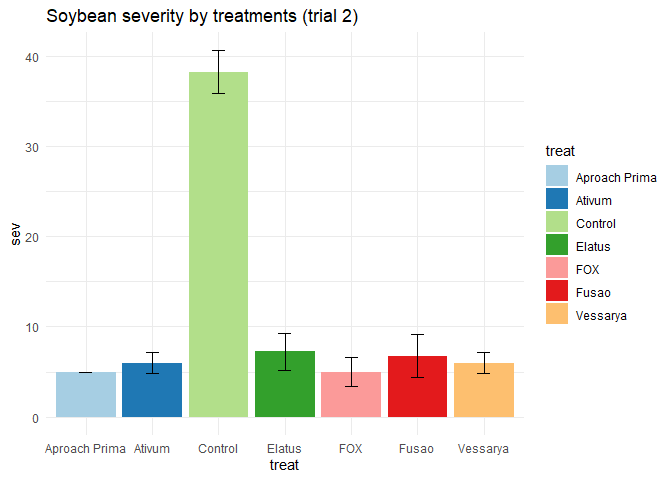
\includegraphics{Trails-of-4-trials_files/figure-latex/dviz2b-1.pdf} The
above table shows that Control(38.25) and treatments; Elatus(7.25) and
Fusao(6.75) had the highest severity.

\hypertarget{data-visualization-for-trial-3}{%
\subsubsection{Data visualization for trial
3}\label{data-visualization-for-trial-3}}

\begin{verbatim}
##           treat     yld        sd
## 1 Aproach Prima 3720.00 444.60994
## 2        Ativum 3719.50 276.85917
## 3       Control 3404.25 501.13962
## 4        Elatus 3421.50 319.41666
## 5           FOX 3718.75  89.92358
## 6         Fusao 3708.75  49.07392
## 7      Vessarya 3790.25 390.76538
\end{verbatim}

The above table shows that treatments; Vessarya(3790.25), Aproach
Prima(3720.00) and Ativum (3719.50) had the highest yield.

\begin{verbatim}
##           treat   sev       sd
## 1 Aproach Prima 26.50 2.380476
## 2        Ativum 21.25 2.500000
## 3       Control 67.50 5.000000
## 4        Elatus 43.75 6.291529
## 5           FOX 20.00 4.082483
## 6         Fusao 22.50 8.660254
## 7      Vessarya 25.00 0.000000
\end{verbatim}

The above table shows that Control(67.50) and treatments; Elatus(43.75)
and Aproach Prima(26.50) had the highest severity.

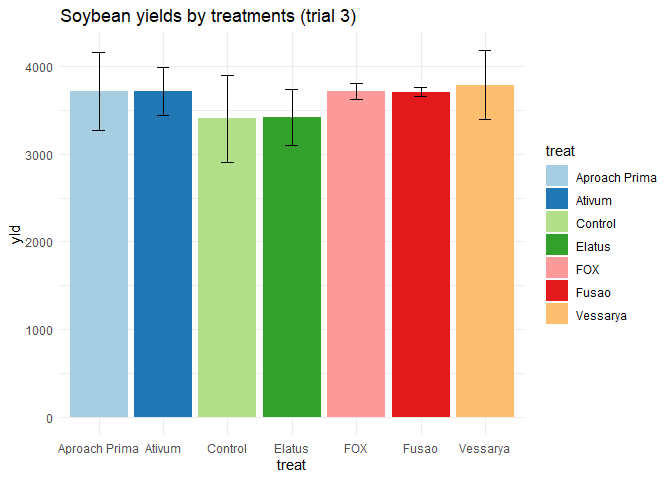
\includegraphics{Trails-of-4-trials_files/figure-latex/dviz3-1.pdf}

The above chart shows that treatments; Vessarya(3790.25), Aproach
Prima(3720.00) and Ativum (3719.50) had the highest yield.

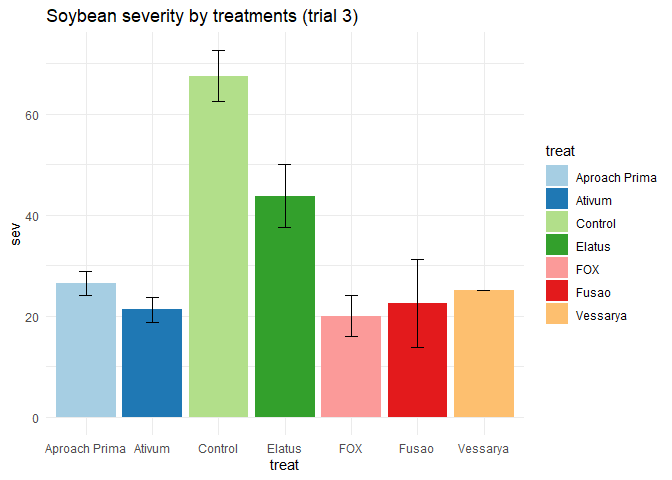
\includegraphics{Trails-of-4-trials_files/figure-latex/dviz3b-1.pdf}

The above chart shows that Control(67.50) and treatments; Elatus(43.75)
and Aproach Prima(26.50) had the highest severity.

\hypertarget{data-visualization-for-trial-4}{%
\subsubsection{Data visualization for trial
4}\label{data-visualization-for-trial-4}}

\begin{verbatim}
##           treat     yld       sd
## 1 Aproach Prima 4133.75 211.1988
## 2        Ativum 4199.25 189.2113
## 3       Control 3363.00 215.0612
## 4        Elatus 3951.50 292.6722
## 5           FOX 4644.25 201.2550
## 6         Fusao 4155.25 467.4551
## 7      Vessarya 4130.00 344.1928
\end{verbatim}

The above table shows that treatments; FOX(4644.25), Ativum (4199.25)
and Ativum (4155.25) had the highest yield in trial 4.

\begin{verbatim}
##           treat   sev        sd
## 1 Aproach Prima 37.00  6.271629
## 2        Ativum 35.75 10.904892
## 3       Control 93.75  2.500000
## 4        Elatus 68.75  6.291529
## 5           FOX 12.00  3.559026
## 6         Fusao 37.00  9.273618
## 7      Vessarya 47.00  6.271629
\end{verbatim}

The above table shows that Control(93.75) and treatments; Elatus(68.75)
and Vessarya(47.00) had the highest severity.

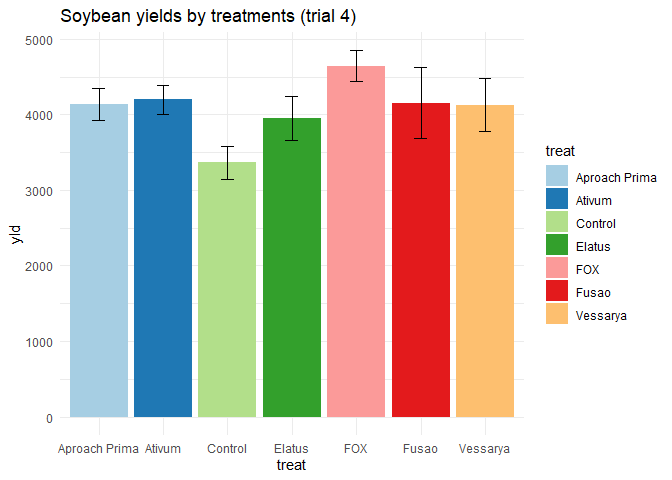
\includegraphics{Trails-of-4-trials_files/figure-latex/dviz4-1.pdf}

The above table shows that treatments; FOX(4644.25), Ativum (4199.25)
and Ativum (4155.25) had the highest yield in trial 4.

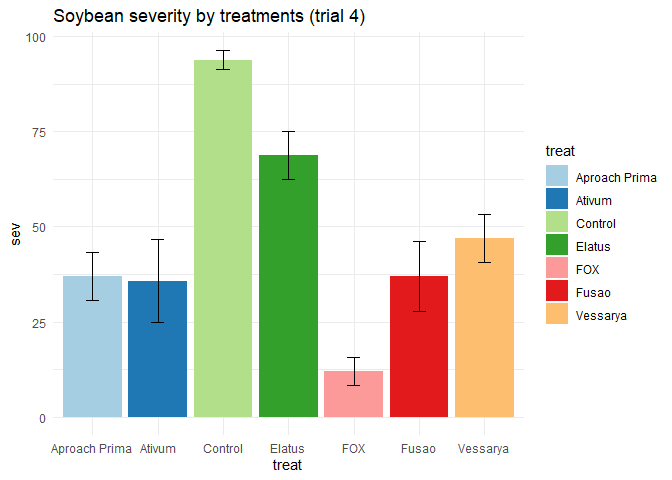
\includegraphics{Trails-of-4-trials_files/figure-latex/dviz4b-1.pdf}

The above chart shows that Control(93.75) and treatments; Elatus(68.75)
and Vessarya(47.00) had the highest severity.

\hypertarget{test-hypotheses-on-the-apparent-effects-for-each-trial}{%
\subsection{10. Test hypotheses on the apparent effects for each
trial}\label{test-hypotheses-on-the-apparent-effects-for-each-trial}}

The one-way analysis of variance (ANOVA), also known as one-factor
ANOVA, is an extension of independent two-samples t-test for comparing
means in a situation where there are more than two groups. In one-way
ANOVA, the data is organized into several groups base on one single
grouping variable (also called factor variable). This tutorial describes
the basic principle of the one-way ANOVA test and provides practical
anova test examples in R software.

The one-way analysis of variance (ANOVA), also known as one-factor
ANOVA, is an extension of independent two-samples t-test for comparing
means in a situation where there are more than two groups. In one-way
ANOVA, the data is organized into several groups base on one single
grouping variable (also called factor variable). This tutorial describes
the basic principle of the one-way ANOVA test and provides practical
anova test examples in R software.

A one-way anova test will be carried out as it is used to evaluate
simultaneously the effect of two grouping variables (A and B) on a
response variable. In this case, the grouping variables are block and
treats while, the response variables are yield and severity.

\hypertarget{hypothesis-testing-for-trial-1}{%
\subsubsection{Hypothesis testing for Trial
1}\label{hypothesis-testing-for-trial-1}}

\hypertarget{hypothesis-testing-for-yield-trial-1}{%
\paragraph{Hypothesis testing for yield (Trial
1)}\label{hypothesis-testing-for-yield-trial-1}}

Null hypothesis: the soybean yield means of the different treatments are
the same.

Alternative hypothesis: At least one treatment means of the soybean
yield is not equal to the others.

\begin{verbatim}
## 
## Call:
## lm(formula = yld ~ treat, data = trl1)
## 
## Coefficients:
##   (Intercept)    treatAtivum   treatControl    treatElatus       treatFOX  
##        3095.2          405.8         -170.0          188.0          310.5  
##    treatFusao  treatVessarya  
##         350.3          152.0
\end{verbatim}

\begin{verbatim}
## Analysis of Variance Table
## 
## Response: yld
##           Df  Sum Sq Mean Sq F value   Pr(>F)    
## treat      6 1010590  168432  6.5739 0.000507 ***
## Residuals 21  538045   25621                     
## ---
## Signif. codes:  0 '***' 0.001 '**' 0.01 '*' 0.05 '.' 0.1 ' ' 1
\end{verbatim}

As the p-value is less than the significance level 0.01, we can conclude
that there are significant differences between the groups highlighted
with ``**" in the anova table. We will also reject the null hypothesis
which states The treatments has no effects on the soybean yield.

\hypertarget{hypothesis-testing-for-severity-trial-1}{%
\paragraph{Hypothesis testing for severity (Trial
1)}\label{hypothesis-testing-for-severity-trial-1}}

Null Hypothesis: The treatments has no effects on the soybean severity.

Alternate Hypothesis: The treatments has effects on the soybean
severity.

\begin{verbatim}
## 
## Call:
## lm(formula = sev ~ treat, data = trl1)
## 
## Coefficients:
##   (Intercept)    treatAtivum   treatControl    treatElatus       treatFOX  
##         38.25           1.25          27.25          -8.75          -4.75  
##    treatFusao  treatVessarya  
##         -8.75         -10.00
\end{verbatim}

\begin{verbatim}
## Analysis of Variance Table
## 
## Response: sev
##           Df Sum Sq Mean Sq F value    Pr(>F)    
## treat      6 4071.2  678.54  14.328 1.825e-06 ***
## Residuals 21  994.5   47.36                      
## ---
## Signif. codes:  0 '***' 0.001 '**' 0.01 '*' 0.05 '.' 0.1 ' ' 1
\end{verbatim}

As the p-value is less than the significance level 0.001, we can
conclude that there are significant differences between the groups
highlighted with ``***" in the anova table. We will also reject the null
hypothesis which states The treatments has no effects on the soybean
severity.

\hypertarget{hypothesis-testing-for-trial-2}{%
\subsubsection{Hypothesis testing for Trial
2}\label{hypothesis-testing-for-trial-2}}

\hypertarget{hypothesis-testing-for-yield-trial-2}{%
\paragraph{Hypothesis testing for yield (Trial
2)}\label{hypothesis-testing-for-yield-trial-2}}

Null hypothesis: the soybean yield means of the different treatments are
the same.

Alternative hypothesis: At least one treatment means of the soybean
yield is not equal to the others.

\begin{verbatim}
## 
## Call:
## lm(formula = yld ~ treat, data = trl2)
## 
## Coefficients:
##   (Intercept)    treatAtivum   treatControl    treatElatus       treatFOX  
##        4114.3         -118.5          -91.0         -202.0           43.0  
##    treatFusao  treatVessarya  
##         -50.5          117.7
\end{verbatim}

\begin{verbatim}
## Analysis of Variance Table
## 
## Response: yld
##           Df Sum Sq Mean Sq F value Pr(>F)
## treat      6 273708   45618  1.0235 0.4374
## Residuals 21 936010   44572
\end{verbatim}

As the p-value = 0.4374 which is greater than the significance level
0.05, we can conclude that there are no significant differences between
the groups highlighted with ``*" in the model summary. we will also
accept the null hypothesis; the soybean yield means of the different
treatments are the same.

\hypertarget{hypothesis-testing-for-severity-trial-2}{%
\paragraph{Hypothesis testing for severity (Trial
2)}\label{hypothesis-testing-for-severity-trial-2}}

Null Hypothesis: The treatments has no effects on the soybean severity.

Alternate Hypothesis: The treatments has effects on the soybean
severity.

\begin{verbatim}
## 
## Call:
## lm(formula = sev ~ treat, data = trl2)
## 
## Coefficients:
##   (Intercept)    treatAtivum   treatControl    treatElatus       treatFOX  
##     5.000e+00      1.000e+00      3.325e+01      2.250e+00     -8.333e-15  
##    treatFusao  treatVessarya  
##     1.750e+00      1.000e+00
\end{verbatim}

\begin{verbatim}
## Analysis of Variance Table
## 
## Response: sev
##           Df Sum Sq Mean Sq F value    Pr(>F)    
## treat      6 3582.4  597.07  201.42 < 2.2e-16 ***
## Residuals 21   62.2    2.96                      
## ---
## Signif. codes:  0 '***' 0.001 '**' 0.01 '*' 0.05 '.' 0.1 ' ' 1
\end{verbatim}

As the p-value is less than the significance level 0.001, we can
conclude that there are significant differences between the groups
highlighted with ``***" in the anova table. We will also reject the null
hypothesis which states The treatments has no effects on the soybean
severity.

\hypertarget{hypothesis-testing-for-trial-3}{%
\subsubsection{Hypothesis testing for Trial
3}\label{hypothesis-testing-for-trial-3}}

\hypertarget{hypothesis-testing-for-yield-trial-3}{%
\paragraph{Hypothesis testing for yield (Trial
3)}\label{hypothesis-testing-for-yield-trial-3}}

Null hypothesis: the soybean yield means of the different treatments are
the same.

Alternative hypothesis: At least one treatment means of the soybean
yield is not equal to the others.

\begin{verbatim}
## 
## Call:
## lm(formula = yld ~ treat, data = trl3)
## 
## Coefficients:
##   (Intercept)    treatAtivum   treatControl    treatElatus       treatFOX  
##       3720.00          -0.50        -315.75        -298.50          -1.25  
##    treatFusao  treatVessarya  
##        -11.25          70.25
\end{verbatim}

\begin{verbatim}
## Analysis of Variance Table
## 
## Response: yld
##           Df  Sum Sq Mean Sq F value Pr(>F)
## treat      6  598170   99695  0.8826 0.5246
## Residuals 21 2372067  112956
\end{verbatim}

As the p-value = 0.5246 which is greater than the significance level
0.05, we can conclude that there are no significant differences between
the groups highlighted with ``*" in the model summary.Therefore, we will
also accept the null hypothesis; the soybean yield means of the
different treatments are the same.

\hypertarget{hypothesis-testing-for-severity-trial-3}{%
\paragraph{Hypothesis testing for severity (Trial
3)}\label{hypothesis-testing-for-severity-trial-3}}

Null Hypothesis: The treatments has no effects on the soybean severity.

Alternate Hypothesis: The treatments has effects on the soybean
severity.

\begin{verbatim}
## 
## Call:
## lm(formula = sev ~ treat, data = trl3)
## 
## Coefficients:
##   (Intercept)    treatAtivum   treatControl    treatElatus       treatFOX  
##         26.50          -5.25          41.00          17.25          -6.50  
##    treatFusao  treatVessarya  
##         -4.00          -1.50
\end{verbatim}

\begin{verbatim}
## Analysis of Variance Table
## 
## Response: sev
##           Df Sum Sq Mean Sq F value    Pr(>F)    
## treat      6 7305.9 1217.65  50.685 2.045e-11 ***
## Residuals 21  504.5   24.02                      
## ---
## Signif. codes:  0 '***' 0.001 '**' 0.01 '*' 0.05 '.' 0.1 ' ' 1
\end{verbatim}

As the p-value is less than the significance level 0.001, we can
conclude that there are significant differences between the groups
highlighted with ``***" in the anova table. We will also reject the null
hypothesis which states The treatments has no effects on the soybean
severity.

\hypertarget{hypothesis-testing-for-trial-4}{%
\subsubsection{Hypothesis testing for Trial
4}\label{hypothesis-testing-for-trial-4}}

\hypertarget{hypothesis-testing-for-yield-trial-4}{%
\paragraph{Hypothesis testing for yield (Trial
4)}\label{hypothesis-testing-for-yield-trial-4}}

Null hypothesis: the soybean yield means of the different treatments are
the same.

Alternative hypothesis: At least one treatment means of the soybean
yield is not equal to the others.

\begin{verbatim}
## 
## Call:
## lm(formula = yld ~ treat, data = trl4)
## 
## Coefficients:
##   (Intercept)    treatAtivum   treatControl    treatElatus       treatFOX  
##       4133.75          65.50        -770.75        -182.25         510.50  
##    treatFusao  treatVessarya  
##         21.50          -3.75
\end{verbatim}

\begin{verbatim}
## Analysis of Variance Table
## 
## Response: yld
##           Df  Sum Sq Mean Sq F value    Pr(>F)    
## treat      6 3496841  582807   6.917 0.0003676 ***
## Residuals 21 1769402   84257                      
## ---
## Signif. codes:  0 '***' 0.001 '**' 0.01 '*' 0.05 '.' 0.1 ' ' 1
\end{verbatim}

As the p-value is less than the significance level 0.001, we can
conclude that there are significant differences between the groups
highlighted with ``***" in the anova table. We will also reject the null
hypothesis which states The treatments has no effects on the soybean
yield.

\hypertarget{hypothesis-testing-for-severity-trial-4}{%
\paragraph{Hypothesis testing for severity (Trial
4)}\label{hypothesis-testing-for-severity-trial-4}}

Null Hypothesis: The treatments has no effects on the soybean severity.

Alternate Hypothesis: The treatments has effects on the soybean
severity.

\begin{verbatim}
## 
## Call:
## lm(formula = sev ~ treat, data = trl4)
## 
## Coefficients:
##   (Intercept)    treatAtivum   treatControl    treatElatus       treatFOX  
##     3.700e+01     -1.250e+00      5.675e+01      3.175e+01     -2.500e+01  
##    treatFusao  treatVessarya  
##     2.284e-14      1.000e+01
\end{verbatim}

\begin{verbatim}
## Analysis of Variance Table
## 
## Response: sev
##           Df  Sum Sq Mean Sq F value    Pr(>F)    
## treat      6 16837.9 2806.31  57.425 6.055e-12 ***
## Residuals 21  1026.2   48.87                      
## ---
## Signif. codes:  0 '***' 0.001 '**' 0.01 '*' 0.05 '.' 0.1 ' ' 1
\end{verbatim}

As the p-value is less than the significance level 0.001, we can
conclude that there are significant differences between the groups
highlighted with ``***" in the anova table. We will also reject the null
hypothesis which states The treatments has no effects on the soybean
severity.

\hypertarget{check-the-correlation-between-severity-and-yield-for-each-trial.}{%
\subsection{11. Check the correlation between severity and yield for
each
trial.}\label{check-the-correlation-between-severity-and-yield-for-each-trial.}}

If the p-value is \textless{} 5\%, then the correlation between x and y
is significant.

\hypertarget{visualizing-the-correlation-between-severity-and-yield-using-a-scatter-plot-for-trial-1}{%
\paragraph{Visualizing the correlation between severity and yield using
a scatter plot for Trial
1}\label{visualizing-the-correlation-between-severity-and-yield-using-a-scatter-plot-for-trial-1}}

\begin{verbatim}
## [1] -0.4985777
\end{verbatim}

\begin{verbatim}
## 
##  Pearson's product-moment correlation
## 
## data:  trl1$sev and trl1$yld
## t = -2.9328, df = 26, p-value = 0.006925
## alternative hypothesis: true correlation is not equal to 0
## 95 percent confidence interval:
##  -0.7349484 -0.1541793
## sample estimates:
##        cor 
## -0.4985777
\end{verbatim}

\begin{verbatim}
## `geom_smooth()` using formula 'y ~ x'
\end{verbatim}

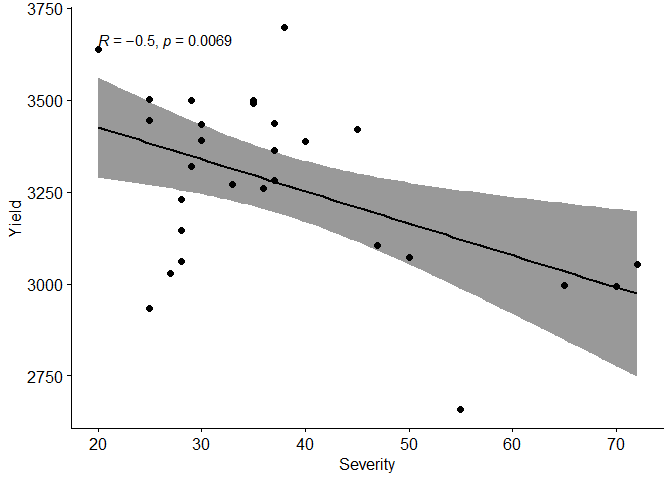
\includegraphics{Trails-of-4-trials_files/figure-latex/cortrl1-1.pdf}
The p-value of the test is 0.006925, which is less than the significance
level alpha = 0.05. We can conclude that severity and yield are
significantly correlated with a correlation coefficient of -0.49837 and
p-value of 0.006925. A correlation coefficient of -0.49837 indicates a
strong negative correlation : this means that every time severity
increases, yield decreases.

\hypertarget{visualizing-the-correlation-between-severity-and-yield-using-a-scatter-plot-for-trial-2}{%
\paragraph{Visualizing the correlation between severity and yield using
a scatter plot for Trial
2}\label{visualizing-the-correlation-between-severity-and-yield-using-a-scatter-plot-for-trial-2}}

\begin{verbatim}
## [1] -0.07672589
\end{verbatim}

\begin{verbatim}
## 
##  Pearson's product-moment correlation
## 
## data:  trl2$sev and trl2$yld
## t = -0.39238, df = 26, p-value = 0.698
## alternative hypothesis: true correlation is not equal to 0
## 95 percent confidence interval:
##  -0.4372857  0.3050840
## sample estimates:
##         cor 
## -0.07672589
\end{verbatim}

\begin{verbatim}
## `geom_smooth()` using formula 'y ~ x'
\end{verbatim}

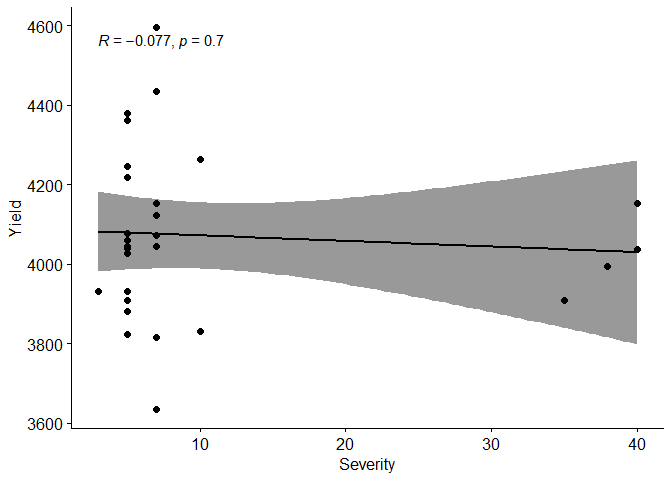
\includegraphics{Trails-of-4-trials_files/figure-latex/cortrl2-1.pdf}
The p-value of the test is 0.698, which is greater than the significance
level alpha = 0.05. We can conclude that severity and yield are not
significantly correlated with a correlation coefficient of -0.07672589
and p-value of 0.698. There is almost no association between the
response variables yield and severity for trial 2.

\hypertarget{visualizing-the-correlation-between-severity-and-yield-using-a-scatter-plot-for-trial-3}{%
\paragraph{Visualizing the correlation between severity and yield using
a scatter plot for Trial
3}\label{visualizing-the-correlation-between-severity-and-yield-using-a-scatter-plot-for-trial-3}}

\begin{verbatim}
## [1] -0.4526989
\end{verbatim}

\begin{verbatim}
## 
##  Pearson's product-moment correlation
## 
## data:  trl3$sev and trl3$yld
## t = -2.5888, df = 26, p-value = 0.01557
## alternative hypothesis: true correlation is not equal to 0
## 95 percent confidence interval:
##  -0.70646059 -0.09580208
## sample estimates:
##        cor 
## -0.4526989
\end{verbatim}

\begin{verbatim}
## `geom_smooth()` using formula 'y ~ x'
\end{verbatim}

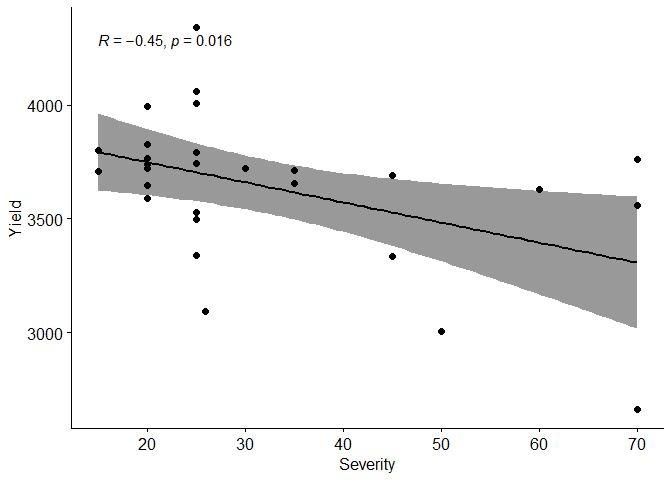
\includegraphics{Trails-of-4-trials_files/figure-latex/cortrl3-1.pdf}
The p-value of the test is 0.01557, which is less than the significance
level alpha = 0.05. We can conclude that severity and yield are
significantly correlated with a correlation coefficient of -0.4526989
and p-value of 0.01557. A correlation coefficient of -0.4526989
indicates a strong negative correlation : this means that every time
severity increases, yield decreases for trial 3.

\hypertarget{visualizing-the-correlation-between-severity-and-yield-using-a-scatter-plot-for-trial-4}{%
\paragraph{Visualizing the correlation between severity and yield using
a scatter plot for Trial
4}\label{visualizing-the-correlation-between-severity-and-yield-using-a-scatter-plot-for-trial-4}}

\begin{verbatim}
## [1] -0.713965
\end{verbatim}

\begin{verbatim}
## 
##  Pearson's product-moment correlation
## 
## data:  trl4$sev and trl4$yld
## t = -5.1994, df = 26, p-value = 1.987e-05
## alternative hypothesis: true correlation is not equal to 0
## 95 percent confidence interval:
##  -0.8583962 -0.4646556
## sample estimates:
##       cor 
## -0.713965
\end{verbatim}

\begin{verbatim}
## `geom_smooth()` using formula 'y ~ x'
\end{verbatim}

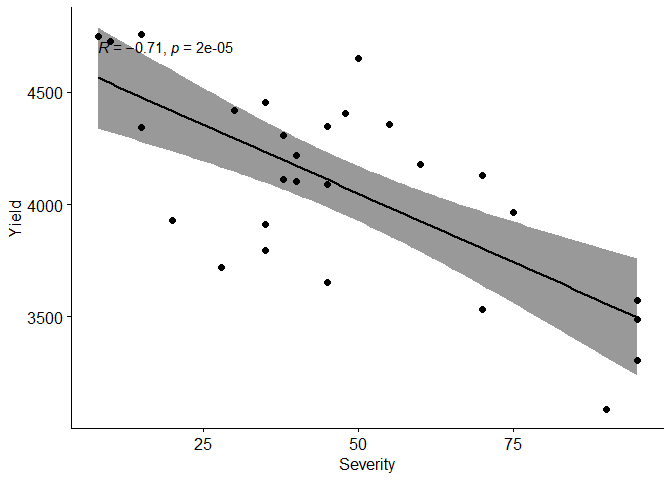
\includegraphics{Trails-of-4-trials_files/figure-latex/cortrl4-1.pdf}

The p-value of the test is 1.987e-05, which is less than the
significance level alpha = 0.05. We can conclude that severity and yield
are significantly correlated with a correlation coefficient of -0.713965
and p-value of 1.987e-05. A correlation coefficient of -0.4526989
indicates a strong negative correlation : this means that every time
severity increases, yield decreases for trial 3.

\end{document}
